\documentclass{beamer} 

% Michael Maier, 2014.
% CC-BY-SA

\usepackage[utf8]{inputenc}
\usepackage[ngerman]{babel}

\title{OpenStreetMap - The Free Wiki World Map} 
\author{Michael Maier \textless Michael.Maier@student.tugraz.at\textgreater} 
\date{September 3rd, 2014} 

\usetheme{Antibes}

\hypersetup{colorlinks=true,urlcolor=blue,linkcolor=white}

%\usebackgroundtemplatei{
%
\includegraphics[width=\paperwidth,
%height=0.8\paperheight]{mag_map.png}
%}

\begin{document}

%\maketitle

\begin{frame} 


\begin{figure}
  \centering
  
\includegraphics[width=.5\textwidth]{mag_map.png}
\end{figure}

\begin{center}
\Huge{OpenStreetMap\\}
\end{center}

\begin{center}
\Large{\emph{The Free Wiki World Map}}
\end{center}

\end{frame}



%\begin{frame}{whoami}
%
%  \begin{itemize}
%    \item Michael Maier \textless \href{mailto:Michael.Maier@student.tugraz.at}{Michael.Maier@student.tugraz.at}\textgreater
%    \item Student of Telematics at Graz University of Technology since 2003
%    \item Involved in Open Source since 2004
%    \item OpenStreetMap since July 2010
%    \item Organising the user group Graz since May 2011
%    \item Talks, workshops and freelance work around OpenStreetMap 
%%    \begin{itemize}
%%      \item OSM-username: \emph{\href{http://www.openstreetmap.org/user/species}{species}}
%%      \item Mapping-area Graz, Leoben on bicycle, motorbike or on public transport
%%    \end{itemize}
%  \end{itemize}
%\end{frame}

\section{Introduction}

\begin{frame}{What is OpenStreetMap}

\begin{itemize}
  \item OpenStreetMap (OSM) is a free world map based on the 'Wiki'-principle
  \begin{itemize}
    \item \emph{Technically, it's a spatial database and not a map}
  \end{itemize}
  \item Based on the work of \textgreater 1.5\,M hobbyist cartographers ``\emph{Mappers}''
%  \item The complete ``planet file''  contains 386 \,GB of data (xml)
      \pause
  \item Licence: Open Database Licence: Think of CC-BY-SA for Data.
\end{itemize}

\begin{center}
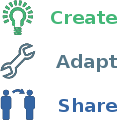
\includegraphics[width=1cm]{ODbL.png}
\hspace{2cm}

\includegraphics[width=1.5cm]{cc-by-sa.png}
\end{center}

\end{frame}

\begin{frame}{Why OpenStreetMap}
	Reasons for creating an Open Streetmap:
\begin{itemize}
  \item There were no free geodata
  \item Usage of existing maps is expensive
  \item Accurancy of existing maps, errors? 
  \item Creating your own styled map
\end{itemize}


\end{frame}

\section{OSM for Transformap}

\begin{frame}{What do we need?}
	A worldwide standardised system, benefits:
\begin{itemize}
  \item One schema (taxonomy), one API
  \item Only one account, whereever in the world
  \item We need to work in parallel
  \item Centralised DB: if one project is abandoned, the data is preserved
\end{itemize}
\end{frame}

\begin{frame}{Benefits of OpenStreetMap}

\begin{itemize}
  \item OSM is independet, run by the OSM Foundation
  \item Data is free - if the foundation collapses, everyone can restart the project
  \item Proven infrastructure of 100\% Free Software
  \item Backed by an active scientific community
  \item Dynamic ecosystem of applications and supporters
  \item Large community, error correction through "wisdom of the crowd"
  \item A lot of data is already there - mostly additions needed
\end{itemize}

\end{frame}


\begin{frame}{Help}

\begin{itemize}
  \item First place should be the wiki:\url{http://wiki.openstreetmap.org}
  \item For questions: $\Rightarrow$ mailing lists!
\item If it exists in your town: the local user group meeting! see \href{http://usergroups.openstreetmap.de/}{openstreetmap.de}.
\end{itemize}

\end{frame}

\section{Thanks for your patience!}

\begin{frame}{The last Slide}

  Slides for Degrowth conference, Leipzig 2014
\vspace{0.7cm}

License of slides: 
\includegraphics[width=1cm]{cc-by-sa.png}.
\vspace{0.7cm}

Created with \LaTeX Beamer, source on \href{https://github.com/species/slides-osm-degrowth}{Github}.
\vspace{0.7cm}

Michael Maier \href{mailto:michael.maier@student.tugraz.at}{Michael.Maier@student.tugraz.at}

Twitter: \href{https://twitter.com/osmgraz}{@osmgraz}

\vspace{0.7cm}
Far more comprehensive slides (german only) from the Mapping Meetup Munich can be downloaded \href{https://github.com/species/vortrag-osm-mmm/blob/master/vortrag.pdf}{here (PDF)}.

\end{frame}

\end{document}
